\chapter{Evaluation}

With an implementation of Multi--Paxos having been developed it is necessary to evaluate it, both in terms of its ability to perform under the assumptions of the environment in which it operates and also to characterise its performance in a number of typical cases.

%%%%%%%%%%%%%%%%%%%%%%%%%%%%%%%%%%%%%%%%%%%%%%%%%%%%%%%%%%%%%%%%%%%%%%%%%%%%%%%%%%%%%%%%%%%%%%%%%%%%%%%%%%%%%%%%%%

\section{Experimental setup}
\label{section:setup}

This section describes the framework upon which simulations were setup to allow for evaluation to take place.

\subsection{Experimental measurements}

Performance evaluation requires the measurement and subsequent analysis of experimental data. There are two key metrics required for evaluating the performance of networked systems -- \emph{latency} and \emph{throughput}. \\

\textbf{Latency} is the time taken elapsed  between a client sending a request to the system and receiving a response. It is measured by a client broadcasting a command with a \texttt{Nop} operation to the set of replicas and starting a timer. The timer is stopped when the response with the corresponding command identifier is received and the elapsed time is calculated and output to a trace log file. \\

\textbf{Throughput} is the rate at which the system services requests and hence measured in requests per unit of time. Clients submit requests at a fixed rate (e.g. 10 requests per second) and the number of responses returned per second is measured by clients. This gives a throughput for a given arrival rate and allows for a \emph{peak throughput} measurement to be made. That is, a certain arrival rate of requests will maximise the output throughput which represents the maximal rate at which the system services requests. \\

\subsection{Mininet}

Mininet is the network simulator that was used for the evaluation of the implementation, running a virtual machine with a Linux guest operating system with 2GB of memory. Mininet ships with a Python API that allows for scripts to run network simulations. Mininet allows for arbitrary Linux processes to be run on any of the virtual hosts. This involved installing an OCaml runtime to execute bytecode compiled on the development machine. The simulation runs Python scripts that performs simulations that proceeds as follows

\begin{enumerate}
  \item Setup up network topology, populating it with hosts and switches and their interconnects (and the performance parameters)
  \item For a given number of each role participating, a JSON configuration file is generated that lists each host IP address and port number
  \item Multi--Paxos instances are started via the OCaml runtime on each virtual host with their parameters set (e.g. whether they are clients)
  \item The simulation starts and proceeds to execute for a given amount of time
  \item The simulation is terminated. Configuration files are deleted and the virtual network is torn down and each process is terminated.
\end{enumerate}

Log files are saved by each process on a shared filesystem with the host machine upon which they are analysed by another Python script which produces plots using matplotlib\footnote{https://matplotlib.org/}. \\

Unless otherwise stated each experiment used 1Gbps, 20ms delay links with a $0\%$ packet loss probability\footnote{As Cap'n Proto uses TCP the developed system does not suffer failures from packet loss, rather it will simply introduce further delays caused by retransmissions} and switches with queue sizes of $10^7$ packets. These characteristics were chosen to help prevent properties of the network from dominating measurements of system performance. The topology of the networks used is discussed in \ref{section-topo}.

\subsection{Duelling leaders and the impossibility result}

\begin{figure}
  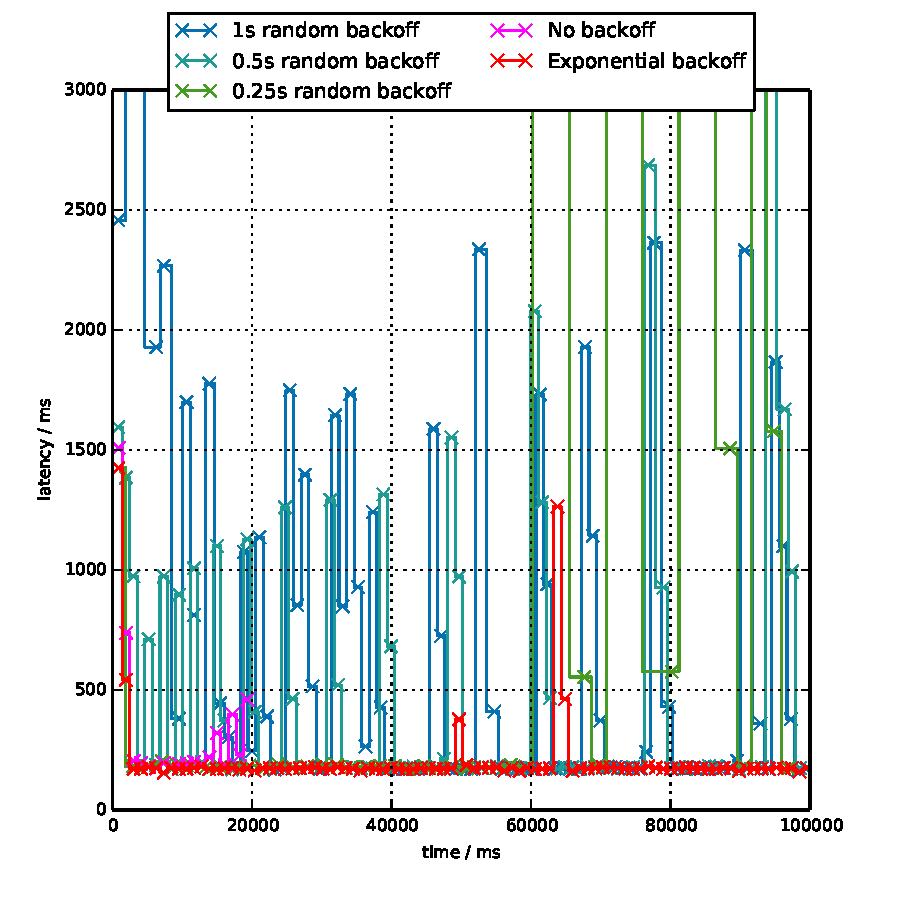
\includegraphics{include/backoffs.pdf}
  \caption{Graph of backoffs}
  \label{fig:backoff-graph}
\end{figure}

When performing initial experiments on the system it became apparent that systems that have more than one leader would regularly livelock when processing requests from clients. Inspection of log files led to me finding out this was a well--known case of \emph{duelling leaders}. This occurs when leaders will attempt to gain adoption of their ballot but are preempted by another leader. The leader will then attempt to gain adoption of another ballot before the other leader's ballot is accepted, causing the other leader to attempt adoption of a higher ballot. The leaders will continually increment their ballots and seek adoption without any given ballot being accept, livelocking the system and leaving it unable to make progress. \\

There is a well known result called the FLP Impossibility result, outlined in Fischer et al's paper \cite{Fischer:1985:IDC:3149.214121} that proves that consensus is never guaranteed in an asynchronous environment that permits crash failures. The problem of duelling leaders is an instance of this problem and so there is no guarantee that consensus can be reached in an asychronous environment. \\

However, there are methods to vastly reduce the chance that leaders will duel. One simple method is to have a \emph{random backoff} so that each leader will pause their operation for a random amount of time in some range. This increases the chance that a leader will have its ballot accepted before being preempted by another leader. A slightly more sophisticated method is to employ \emph{exponential backoff}. In this case each leader will employ a random backoff within some range and upon being preempted this range is doubled. The backoff time is reduced to an initial value when an adopted message is received by a leader. This reduces the amount of idle waiting that may occur when using a random backoff and no duelling is occurring. \\

Figure \ref{fig:backoff-graph} shows a number of traces with different backoff strategies. With no backoff, the system halts after 18 requests are processed and makes no further progress. Three traces of random backoffs with different maximum wait times were collected. With greater maximum wait times there are a number of greater sporadic delays in the system as these leaders often have to wait idly even when duelling is not occuring. Making the random timeout too small, as in the 0.25s case, reduces the number of delays but increases the chance leaders will duel for some time before one waits long enough for the other to make progress, resulting in very large delays. The exponential backoff (starting with a value of 0.25s) performs best, with very little delay in the general case and ocassional delays as backoff windows increase in size when leaders do duel.

\subsection{Topologies}
\label{section-topo}

\begin{figure}[t]
  \centering
  \scalebox{0.7}{ 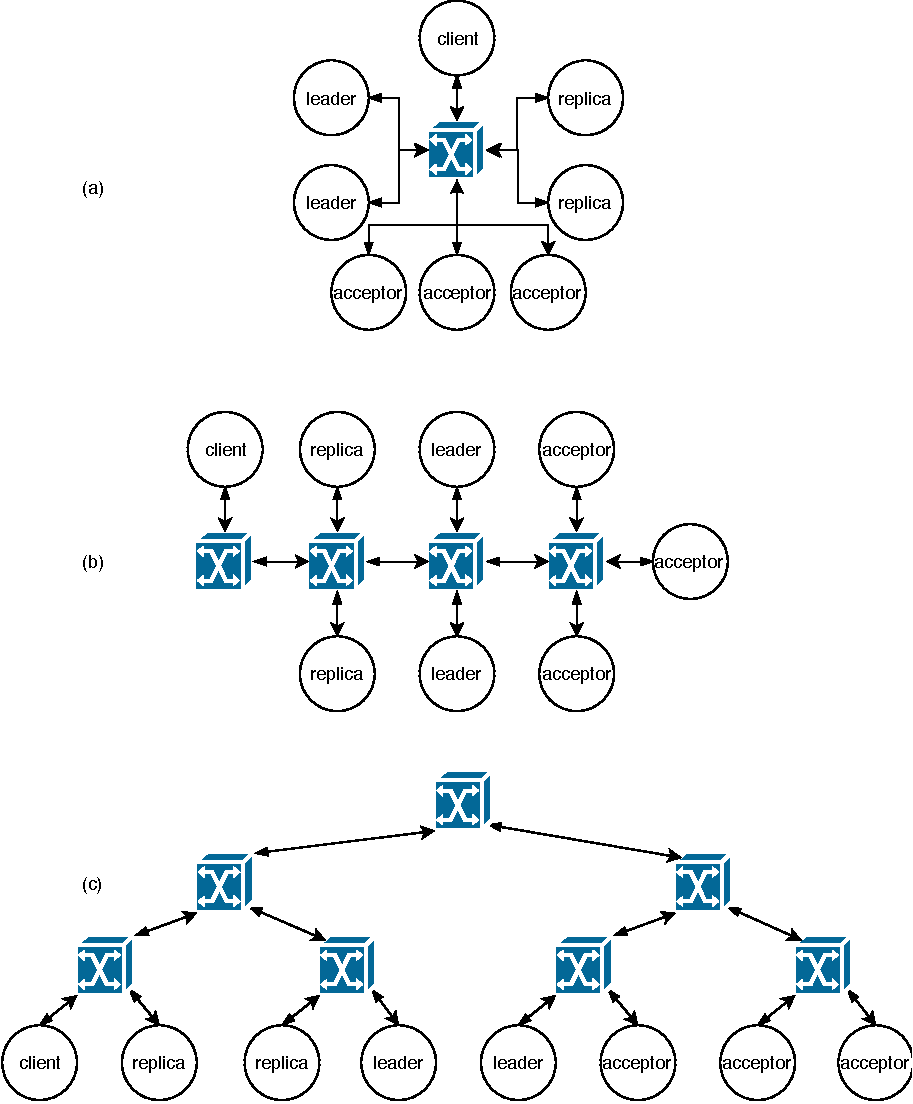
\includegraphics{include/topo-diagram.pdf}}
  \caption{Diagrams of different network topologies investigated. Topology (a) represents a star topology, (b) represents a linear topology and (c) a tree topology.}
  \label{fig:topo-diagram}
\end{figure}

\begin{figure}
  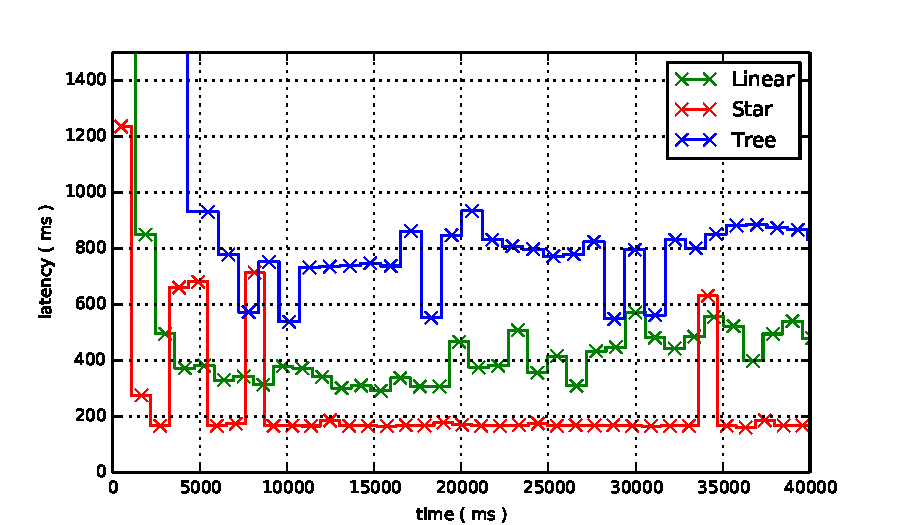
\includegraphics{include/topos.pdf}
  \caption{Graph of latencies over time with different network topologies.}
  \label{fig:topo-graph}
\end{figure}

An important consideration when evaluating the system on a simulated network is to ensure that the results collected do not reflect the characteristics of the network itself rather than reflecting the characteristics of the system itself. For example we do not wish for delays in queues at switches to dominate the measurements of latency for the system itself. An initial experiment was performed to observe the steady state behaviour of the system with three different network topologies, shown in Figure \ref{fig:topo-diagram}. A client submit requests to the replicas every 1.0s and the latency of these requests is measured. Topology (a) represents a star topology wherein each host is connected to a single switch. Topology (b) represents a linear network wherein each process with the same role is connected to a single switch and these are each connected together. Topology (c) represents a tree topology with switches arranged in a binary tree structure. \\

Figure \ref{fig:topo-graph} shows the traces produced when measuring the steady state latency of each topology. No unexpected behaviour occurs in any of the three schemes. The main difference to note is that the average latency of each trace varies between each topology. This is because the number of hops from each sender and receiver participating in the system varies. For example, every pair of hosts that need to communicate is two hops away in the star topology, 3 hops away in the linear topology and a variable number of hops away in the tree topology. There is no unexpected queuing behaviour resulting in very large delays for any of the given topologies. \\

%%%%%%%%%%%%%%%%%%%%%%%%%%%%%%%%%%%%%%%%%%%%%%%%%%%%%%%%%%%%%%%%%%%%%%%%%%%%%%%%%%%%%%%%%%%%%%%%%%%%%%%%%%%%%%%%%%

%{\color{green}\section{Simulation tests}

%Define here what we  meanby simulation tests: tests that ensure the expected behaviour of the system as a whole is undertaken. \\

%Explain this fits into our definitions of what a test harness is and how we're going to use that to perform evaluations. Explain this also requires modification of the program to ensure we can crash / delay acceptors suitably so as to simulate the sort of failure modes we require. \\

%Perhaps describe a system test and then also reference a table describing each test in the appendix. \\}

%%%%%%%%%%%%%%%%%%%%%%%%%%%%%%%%%%%%%%%%%%%%%%%%%%%%%%%%%%%%%%%%%%%%%%%%%%%%%%%%%%%%%%%%%%%%%%%%%%%%%%%%%%%%%%%%%


\section{Performance evaluation}

The performance evaluation explores two key areas. The first is how the latency and throughput of the system change as the number of processes participating in the protocol grows. The second is how these performance metrics change in the face of failures.

\subsection{System size}

It is important to characterise the behaviour of the system as the number of processes is varied. For these experiments the number of each role is fixed in a system with 1 client and $f = 1$; that is 2 replicas, 2 leaders, 3 acceptors. Then for each experiment the number of each process was increased and the latency and throughput observed.

%For the first three experiments the number of each role is fixed in a system with 1 client and $f = 1$; that is 2 replicas, 2 leaders, 3 acceptors. Then for each experiment the number of each process was increased and the latency and throughput observed. In the next experiment $f$ was varied so the number of each role is increased proportionally with the number of failures tolerated.

\subsubsection{Method}

For each system size we wish to characterise the average latency and throughput in the steady state. For this experiment the system was arranged in a star topology, with the network parameters described in \label{section:setup}. When collecting latency measurements, clients submit requests every second for 60 seconds. The first 5 seconds of measurements are discarded since they exhibit non--steady--state behaviour. The experiment produces a collection of latencies $\left{t_1, t_2, t_3, \ldots t_N \right}$. The average latency for this trace is the sample mean of these, that is

$$ \bar{t} = \frac{1}{N} \sum^{N}_{n=1} t_n$$

In order to construct a confidence interval, the simulation was repeated $M=5$ times, producing a collection of average latencies $\left{\bar{t}_1, \bar{t}_2, \bar{t}_3, \ldots \bar{t}_M \right}$. The sample mean of these is computed to give $T$, the latency averaged over each run of the simulation 

$$ \bar{T}= \frac{1}{M} \sum^{M}_{m=1} \bar{t}_m$$

and sample variance

$$ \sigma^2 = \frac{1}{M - 1} \sum^{M}_{m=1} \left( \bar{t}_m - \bar{T} \right)^2 $$

This allows us to construct a $95\%$ confidence interval for each experiment, given by

$$ \left[ \bar{T} - \frac{1.96 \ \sigma}{\sqrt{M}}, \ \bar{T} + \frac{1.96 \ \sigma}{\sqrt{M}} \right]$$

\begin{figure}
  \centering
  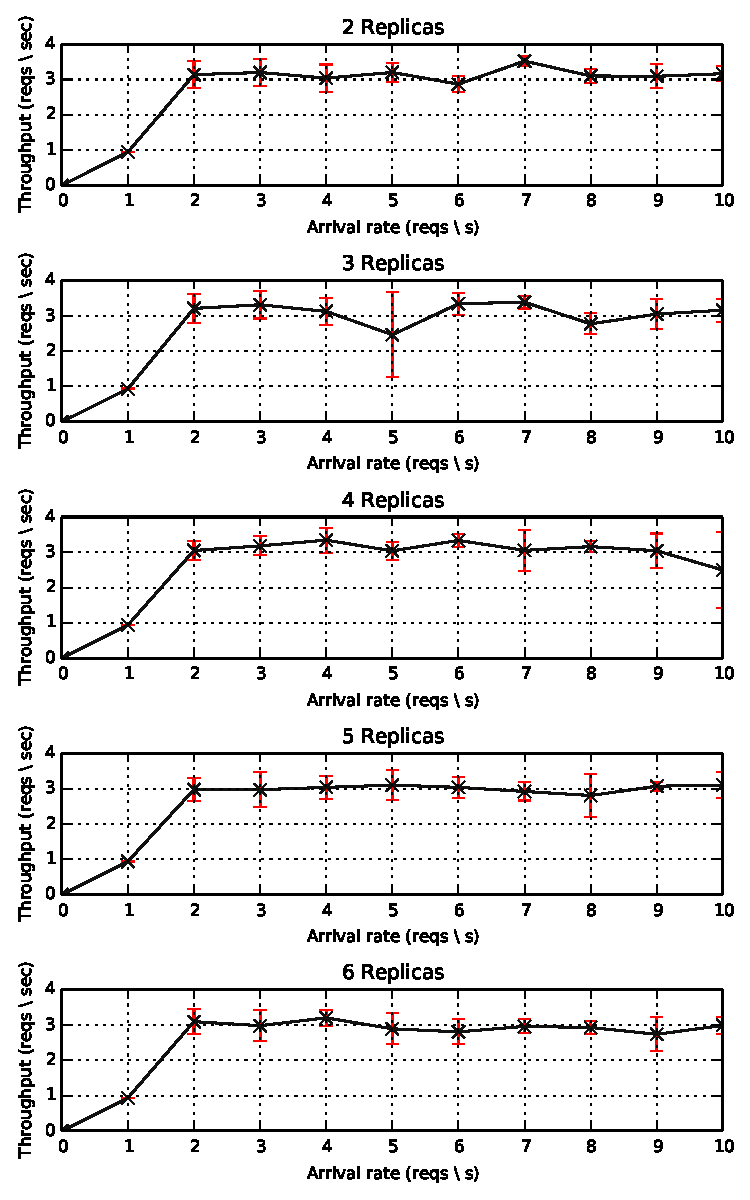
\includegraphics{include/tputs.pdf}
  \caption{Graphs displaying how throughput varies with arrival rate of requests for a number systems with different replica sizes.}
  \label{fig:tput-example}
\end{figure}

The \emph{peak average throughput} was determined for every system size. For each system size, the throughput of the system was measured as the rate of requests from the client, called the arrival rate, was varied. For each arrival rate, the average throughput was computed by dividing the number of responses by the time interval over which they were received. \\

The results of such an experiment produce a set of graphs like those in Figure \ref{fig:tput-example}, which contains how these throughputs vary as the number of replicas is increased. Increasing the sending rate of the client causes the throughput to increase; this is because when the system is under--utilised the faster requests are sent the faster they will be processed. This occurs up to a certain sending rate, wherein the system becomes fully utilised and increasing the sending rate does not increase the throughput but instead causes it to oscillate near the limit or drop slightly as the system becomes overloaded.

\subsubsection{Results}

\begin{figure}[t]
  \centering
  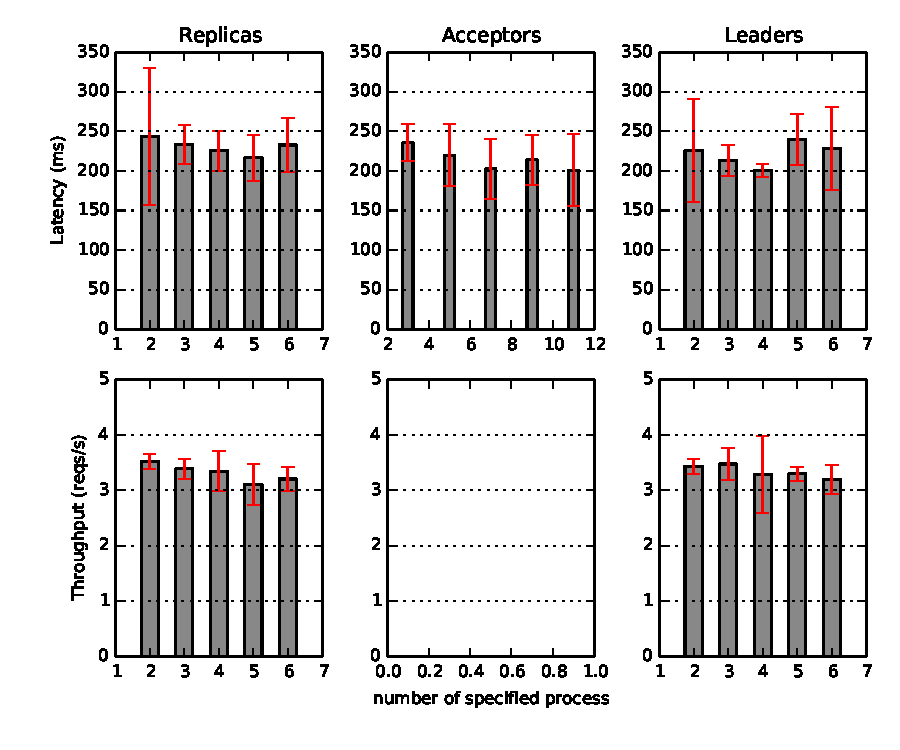
\includegraphics{include/system-size-roles.pdf}
  \caption{Results of latency and throughput as system size was varied for each role separately. For each graph the roles that did not vary were fixed in a system with $f=1$. Error bars show $95\%$ confidence intervals.}
  \label{fig:system-size-roles}
\end{figure}

%\begin{figure}[t]
%  \centering
%  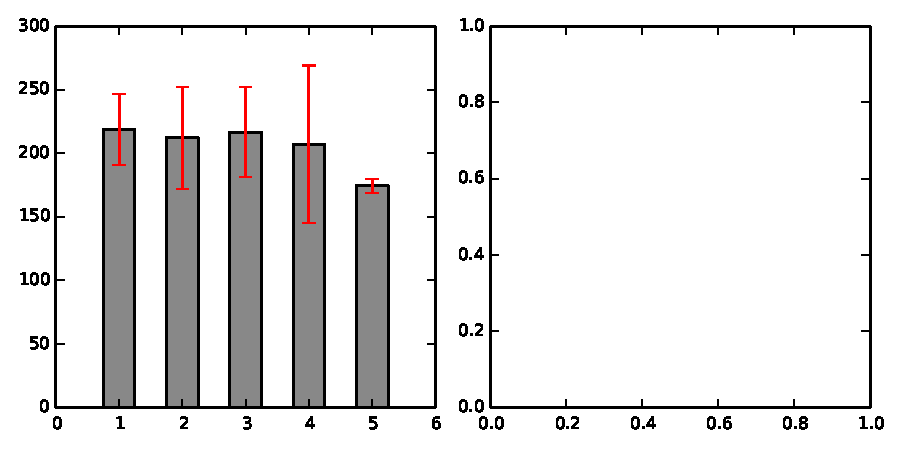
\includegraphics{include/system-size-all.pdf}
%  \caption{Results of latency and throughput as whole system size was varied, in increments of the number of tolerable failures $f$. Error bars show $95\%$ confidence intervals.}
%  \label{fig:system-size}
% \end{figure}

{\color{red}TODO: Do more runs of the throughput simulations to construct confidence intervals. \\}

{\color{red}TODO: Finish analysing acceptor throughputs. \\}

The results of the experiment are displayed in Figure \ref{fig:system-size-roles}. In each case there is no drastic change in latency or throughput of the system as the number of each role is varied. \\

In the general case most replicas will propose the same serialisation of commands to the leaders which are then de--duplicated. Hence increasing the number of replicas does not introduce additional overhead except to increase the number of messages in the network. This does not incur a performance penalty when the network is not congested. The number of leaders exhibits decreasing latency as the system is increased to 4 leaders and then increases again. This unusual behaviour may be attribute to random variations in the simulations rather than the behaviour of the system; as the confidence intervals of each experiment overlap. This is also reflected in the throughput as the system exhibits unusually high throughput for the case of 4 leaders. \\

\subsection{Failure traces}

\begin{figure}
  \centering
  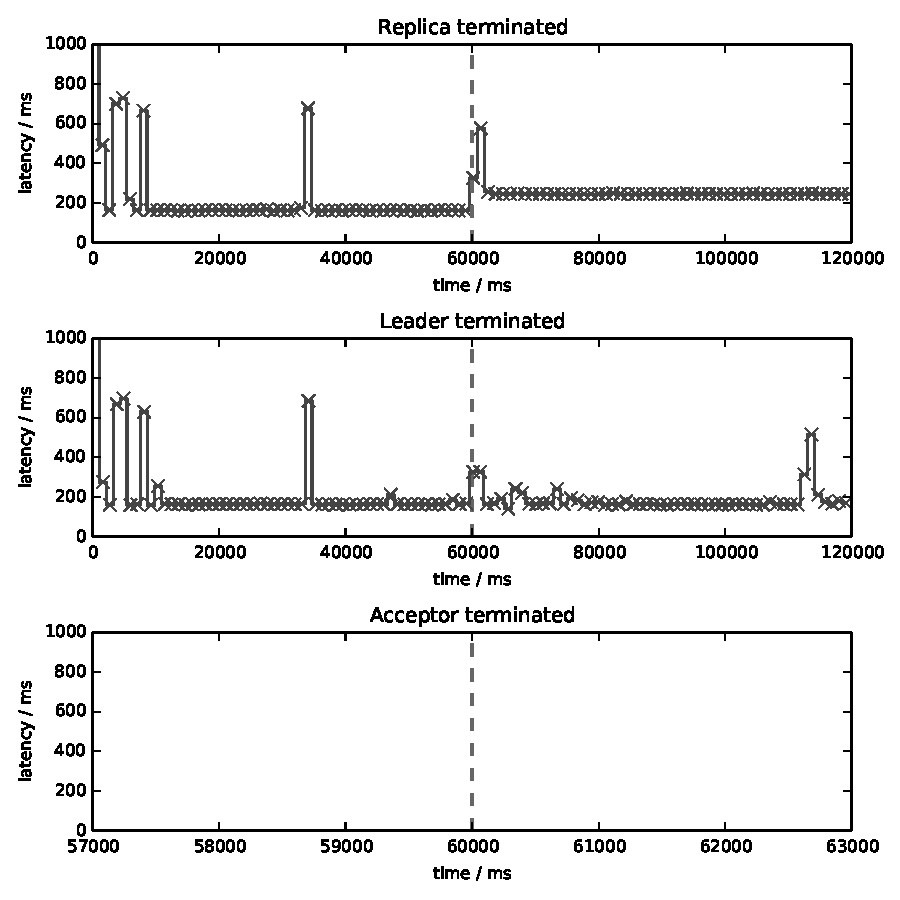
\includegraphics{include/singe-crash-graph.pdf}
  \caption{System size}
  \label{fig:failure-traces}
\end{figure}

This experiment observes the behaviour of the system when failure of a process is triggered. Each simulation ran for 120 seconds with a client submitting commands at a rate of 1 per second and a system size with $f=1$. After 60 seconds of simulated time has elapsed a process failure is triggered; this involves the killing of a specific process on a virtual host. The simulation continues to run for another 60 seconds so the behaviour after the failure can be observed. Simulations were performed separately for killing a replica, leader and acceptor. \\

The traces produced are shown in Figure \ref{fig:failure-traces}. In each case the system begins as usual with very high latencies before settling into steady state behaviour. In the case of a replica process failing, there is a transient increase in latency before settling down to a latency higher than before the crash. The leader process failing causes an increase in latency, smaller than that of the replica, and causes small transient delays briefly thereafter. Unlike the replica failure the latency returns to that of before the crash. \\

{\color{red}TODO: Have a look over the acceptor code because it doesn't seem to be behaving as it should. Repeat experiment after.}

%\subsection{Failure traces}
%
%\begin{figure}
%  \centering
%  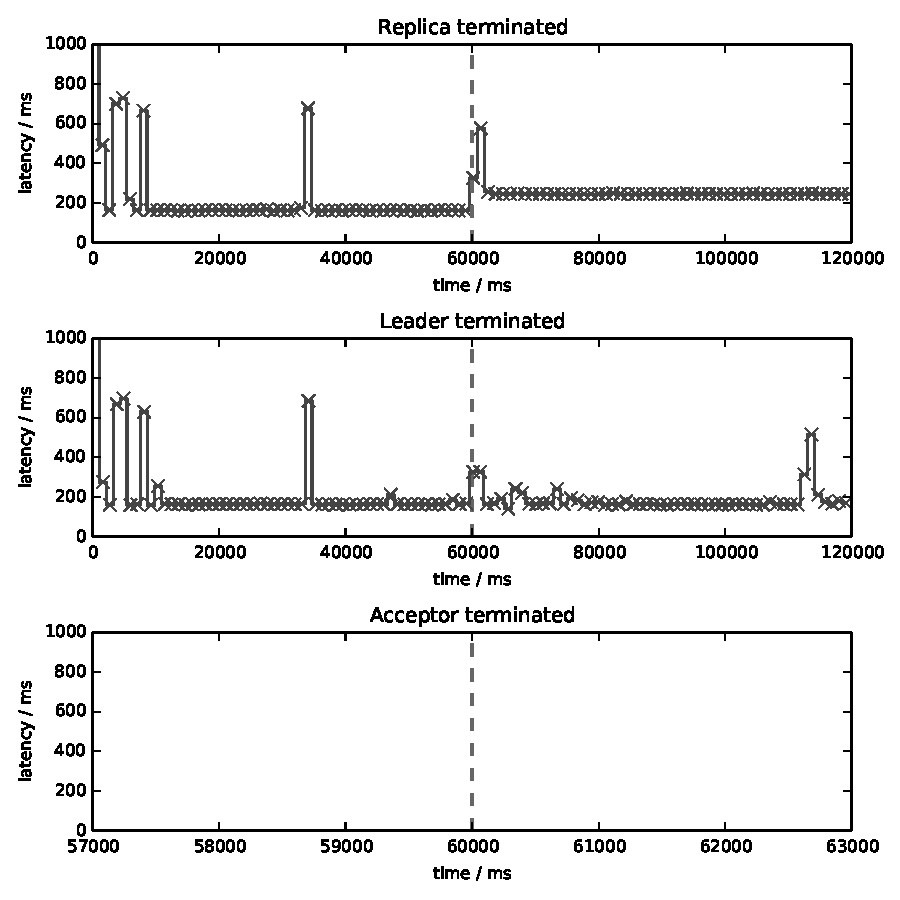
\includegraphics{include/singe-crash-graph.pdf}
%  \caption{System size}
%  \label{fig:system-size}
%\end{figure}

%Describe how we need to assess the system in the case of failures. \\

%{\color{blue}Replica failure traces. Include plain failures, failures including restarts and cascading failure until we get no further latency and throughput. Include LibPaxos traces over the time. %Should result in six graphs if we're lucky.} \\
